\documentclass{article}
\usepackage{amsmath, amssymb, verbatim, amsthm, tikz}
\usetikzlibrary{arrows}
\newcommand{\contradiction}{\Rightarrow\!\Leftarrow}
% I need a title
\author{Minh Bui}
\title{Math 323 HW8}

\theoremstyle{claim}
\newtheorem{claim}{Claim}
\newtheorem{theorem}{Theorem}[section]
\newtheorem{corollary}{Corollary}[theorem]
\newtheorem{lemma}[theorem]{Lemma}
\theoremstyle{definition}
\newtheorem{definition}{Definition}
\begin{document}
% Generates the title
\maketitle
\begin{enumerate}
    \item[Problem 6.*] Prove the \emph{Alternate Completeness axiom}.\\
        We first review our definition of a completed ordered field and the Alternate Completeness Axiom.
        \begin{definition}
            An ordered field $\mathbb{F}$ is completed when: if for any nonempty subset $S$ of $\mathbb{F}$ and $S$ has at least one lower bound, then $\exists s \in \mathbb{F}$ that is the greatest lower bound of $S$.
        \end{definition}
        \begin{theorem}
            \emph{The Alternate Completeness Axiom.} For a completed ordered field $\mathbb{F}$: If $S$ is a nonempty set from $\mathbb{F}$ and $S$ has at least one upper bound, then $\exists u \in \mathbb{F}$ that is the least upper bound of $S$.
        \end{theorem}
        \begin{proof}
            Assume $\mathbb{F}$ is a completed ordered field.\\
            Assume $S$ is a nonempty set from $\mathbb{F}$.\\
            Assume $S$ has at least one upper bound.\\
            We define
            \begin{equation*}
                UB(S) = \{ u \in \mathbb{F} \mid u \text{ is an upper bound of } S \}
            \end{equation*}
            We first want to prove the following
            \begin{lemma}
                If $s \in S$ then $s$ is a lower bound of $UB(S)$.
            \end{lemma}
            \begin{proof}
                Assume $s \in S$. We want to prove: if $u \in UB(S)$, then $u \ge s$.\\
                Assume $u \in UB(S)$, since $UB(S)$ is a set of upper bounds of $S$, we know: if $t \in S$, then $u \ge t$. And so $s$ is a lower bound of $UB(S)$.
            \end{proof}
            We consider $UB(S)$. $UB(S)$ has at least one element by our assumption of $S$ having at least one upper bound. We know $UB(S)$ has at least one lower bound by our lemma. We also know $\mathbb{F}$ is completed. So by the definition of completeness, $\exists g \in \mathbb{F}$ that is the greatest lower bound of $UB(S)$. This means
            \begin{enumerate}
                \item[1.] If $u \in UB(S)$, then $u \ge g$.
                \item[2.] If $x \in \mathbb{F}$ and $x > g$, then $\exists t \in UB(S)$ so that $t < x$.
            \end{enumerate}
            We claim that $g$ is the least upper bound of $S$. This means we have to prove two properties:
            \begin{enumerate}
                \item[1.] If $s \in S$, then $g \ge s$.\\
                    Assume $s \in S$. Since $g$ is the greatest lower bound of $UB(S)$, if $l$ is a lower bound on $UB(S)$, then $g \ge l$. By our lemma, we know if $s \in S$, then $s$ is a lower bound on $UB(S)$. And so $g \ge s$. 
                \item[2.] If $y \in \mathbb{F}$ and $y < g$, then $\exists v \in S$ so that $y < v$.\\
                    We can try to rewrite this statement: If $u$ is an upper bound of $S$, then $g \le u$. Assume $u \in UB(S)$. Since $g$ is the greatest lower bound of $UB(S)$, $u \ge g$.
            \end{enumerate}
            So we have proved that: For a completed ordered field $\mathbb{F}$: If $S$ is a nonempty set from $\mathbb{F}$ and $S$ has at least one upper bound, then $\exists u \in \mathbb{F}$ that is the least upper bound of $S$.

        \end{proof}
    \item[Problem 6.1:] Let $S = \{ x \in \mathbb{R} \mid x^{-1} \in \mathbb{N} \}$. Prove that $0$ is the greatest lower bound of $S$.
        \begin{proof}
            To prove the above statement, we have to establish two properties for $0$.
            \begin{enumerate}
                \item[1.] If $x \in S$, $0 \le x$.\\
                    Since $x^{-1} \in \mathbb{N}$, $x = \frac{1}{n}$ where $n \in \mathbb{N}$. So $x = \frac{1}{n} \ge 0$. This means $0$ is a lower bound of $S$.
                \item[2.] If $x \in \mathbb{R}$ and $x > 0$, then $\exists t \in S$ so that $t < x$.\\
                    Since $S$ is a nonempty set of real numbers and has $0$ as a lower bound, by completeness, $S$ has a greatest lower bound. Assume $x \in \mathbb{R}$ and $x > 0$. We need to prove the following lemma.
                    \begin{lemma}
                        If $r \in \mathbb{R}$ and $r > 0$, then $\exists n \in \mathbb{N}$ so that $\frac{1}{n} < r$.
                    \end{lemma}
                    \begin{proof}
                        Assume $r \in \mathbb{R}$ and $r > 0$. Consider $r^{-1}$. Since $r \in \mathbb{R}$, $r^{-1} \in \mathbb{R}$. By the Archimedean principle, $\exists n \in \mathbb{N}$ so that $n > r^{-1}$. This means
                        \begin{gather*}
                            n > \frac{1}{r}\\
                            nr > 1 \text{ because } r > 0\\
                            r > \frac{1}{n}
                        \end{gather*}
                    \end{proof}
                    The lemma we just proved basically says: For any real number $r$ and $r > 0$, $\exists n$ such that $r > \frac{1}{n}$. \\
                    By our lemma, assume $x \in \mathbb{R}$ and $x > 0$, then $\exists n_0 \in \mathbb{N}$ such that $r > \frac{1}{n_0}$. Let $t = \frac{1}{n_0}$. So $r > t$. But $t \in S$ so we are done.
            \end{enumerate}
        \end{proof}
    \item[Problem 6.2:] Using the notation
        \begin{equation*}
            UB(S) = \{ u \in \mathbb{R} \mid u \text{ is an upper bound on the set } S \}.
        \end{equation*}
        set in the proof of the proof of the alternate completeness axiom, find:
        \begin{enumerate}
            \item $UB(A)$ for $A = \{ x \in \mathbb{R} \mid x < 5 \}$.
            \item[] $UB(A) = \{ u \in \mathbb{R} \mid u \ge 5\}$\\
                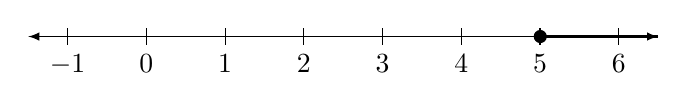
\begin{tikzpicture}
                    \draw[latex-latex] (-1.5, 0) -- (6.5, 0) ;
                    \foreach \x in {-1, 0, 1, 2, 3, 4, 5, 6}
                    \draw[shift={(\x,0)}, color=black] (0pt,3pt) -- (0pt,-3pt);
                    \foreach \x in {-1, 0, 1, 2, 3, 4, 5, 6}
                    \draw[shift={(\x,0)}, color=black] (0pt,0pt) -- (0pt, -3pt) node[below]
                    {$\x$};
                    \draw[*-] (4.92,0) -- (6.5,0);
                    \draw[very thick] (5,0) -- (6.5, 0);
                \end{tikzpicture}
            \item $UB(B)$ for $B = \{ x \in \mathbb{R} \mid x \le 5 \}$.
            \item[] $UB(B) = \{ u \in \mathbb{R} \mid u \ge 5\}$\\
                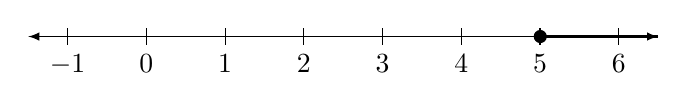
\begin{tikzpicture}
                    \draw[latex-latex] (-1.5, 0) -- (6.5, 0) ;
                    \foreach \x in {-1, 0, 1, 2, 3, 4, 5, 6}
                    \draw[shift={(\x,0)}, color=black] (0pt,3pt) -- (0pt,-3pt);
                    \foreach \x in {-1, 0, 1, 2, 3, 4, 5, 6}
                    \draw[shift={(\x,0)}, color=black] (0pt,0pt) -- (0pt, -3pt) node[below]
                    {$\x$};
                    \draw[*-] (4.92,0) -- (6.5,0);
                    \draw[very thick] (5,0) -- (6.5, 0);
                \end{tikzpicture}
            \item $UB(C)$ for $C = \{ 5 \}$
            \item[] $UB(C) = \{ u \in \mathbb{R} \mid u \ge 5 \}$\\
                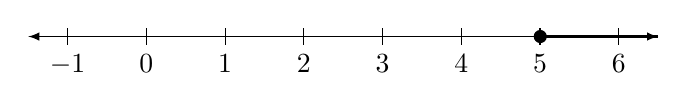
\begin{tikzpicture}
                    \draw[latex-latex] (-1.5, 0) -- (6.5, 0) ;
                    \foreach \x in {-1, 0, 1, 2, 3, 4, 5, 6}
                    \draw[shift={(\x,0)}, color=black] (0pt,3pt) -- (0pt,-3pt);
                    \foreach \x in {-1, 0, 1, 2, 3, 4, 5, 6}
                    \draw[shift={(\x,0)}, color=black] (0pt,0pt) -- (0pt, -3pt) node[below]
                    {$\x$};
                    \draw[*-] (4.92,0) -- (6.5,0);
                    \draw[very thick] (5,0) -- (6.5, 0);
                \end{tikzpicture}
            \item $UB(D)$ for $D = \{ 4, 5, 6 \}$
            \item[] $UB(D) = \{ u \in \mathbb{R} \mid u \ge 6 \}$\\
                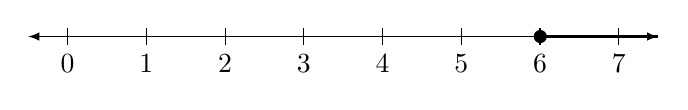
\begin{tikzpicture}
                    \draw[latex-latex] (-0.5, 0) -- (7.5, 0) ;
                    \foreach \x in {0, 1, 2, 3, 4, 5, 6, 7}
                    \draw[shift={(\x,0)}, color=black] (0pt,3pt) -- (0pt,-3pt);
                    \foreach \x in {0, 1, 2, 3, 4, 5, 6, 7}
                    \draw[shift={(\x,0)}, color=black] (0pt,0pt) -- (0pt, -3pt) node[below]
                    {$\x$};
                    \draw[*-] (5.92,0) -- (6.5,0);
                    \draw[very thick] (6,0) -- (7.5, 0);
                \end{tikzpicture}
            \item $UB(E)$ for $E = \{ x \in \mathbb{Z} \mid x < 5\}$
            \item[] $UB(E) = \{ u \in \mathbb{Z} \mid x \ge 5\}$\\
                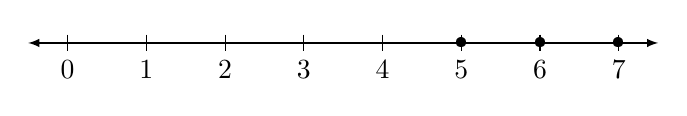
\begin{tikzpicture}
                    \draw[latex-latex] (-0.5, 0) -- (7.5, 0) ;
                    \foreach \x in {0, 1, 2, 3, 4, 5, 6, 7}
                    \draw[shift={(\x,0)}, color=black] (0pt,3pt) -- (0pt,-3pt);
                    \foreach \x in {0, 1, 2, 3, 4, 5, 6, 7}
                    \draw[shift={(\x,0)}, color=black] (0pt,0pt) -- (0pt, -3pt) node[below]
                    {$\x$};
                    \foreach \Point in {(5,0), (6,0), (7, 0)}
                        \node at \Point {\textbullet};
                \end{tikzpicture}
            \item $UB(F)$ for $F = \{ x \in \mathbb{Z} \mid x \le 5\}$
            \item[] $UB(F) = \{ u \in \mathbb{Z} \mid u \ge 5\}$\\
                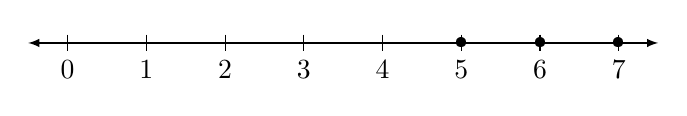
\begin{tikzpicture}
                    \draw[latex-latex] (-0.5, 0) -- (7.5, 0) ;
                    \foreach \x in {0, 1, 2, 3, 4, 5, 6, 7}
                    \draw[shift={(\x,0)}, color=black] (0pt,3pt) -- (0pt,-3pt);
                    \foreach \x in {0, 1, 2, 3, 4, 5, 6, 7}
                    \draw[shift={(\x,0)}, color=black] (0pt,0pt) -- (0pt, -3pt) node[below]
                    {$\x$};
                    \foreach \Point in {(5,0), (6,0), (7, 0)}
                        \node at \Point {\textbullet};
                \end{tikzpicture}
        \end{enumerate}

\end{enumerate}
\end{document}
